%%%%%%%%%%%%%%%%%%%%%%%%%%%%%%%%%%%%%%%%%
% Stylish Article
% LaTeX Template
% Version 2.1 (1/10/15)
%
% This template has been downloaded from:
% http://www.LaTeXTemplates.com
%
% Original author:
% Mathias Legrand (legrand.mathias@gmail.com) 
% With extensive modifications by:
% Vel (vel@latextemplates.com)
%
% License:
% CC BY-NC-SA 3.0 (http://creativecommons.org/licenses/by-nc-sa/3.0/)
%
%%%%%%%%%%%%%%%%%%%%%%%%%%%%%%%%%%%%%%%%%

%----------------------------------------------------------------------------------------
%	PACKAGES AND OTHER DOCUMENT CONFIGURATIONS
%----------------------------------------------------------------------------------------

\documentclass[fleqn,10pt]{SelfArx} % Document font size and equations flushed left

\usepackage[ngerman]{babel} % Specify a different language here - english by default

\usepackage{lipsum} % Required to insert dummy text. To be removed otherwise

\usepackage{verbatim}

\usepackage{listings}
\lstset{language=sql,breaklines=true}

%----------------------------------------------------------------------------------------
%	COLUMNS
%----------------------------------------------------------------------------------------

\setlength{\columnsep}{0.55cm} % Distance between the two columns of text
\setlength{\fboxrule}{0.75pt} % Width of the border around the abstract

%----------------------------------------------------------------------------------------
%	COLORS
%----------------------------------------------------------------------------------------

\definecolor{color1}{RGB}{0,0,90} % Color of the article title and sections
\definecolor{color2}{RGB}{0,20,20} % Color of the boxes behind the abstract and headings

%----------------------------------------------------------------------------------------
%	HYPERLINKS
%----------------------------------------------------------------------------------------

\usepackage{hyperref} % Required for hyperlinks
\hypersetup{hidelinks,colorlinks,breaklinks=true,urlcolor=color2,citecolor=color1,linkcolor=color1,bookmarksopen=false,pdftitle={Title},pdfauthor={Author}}

%----------------------------------------------------------------------------------------
%	ARTICLE INFORMATION
%----------------------------------------------------------------------------------------

\JournalInfo{Journal, Vol. XXI, No. 1, 1-5, 2013} % Journal information


\PaperTitle{Datenbanken} % Article title

\Authors{Carlo Hamann}

%----------------------------------------------------------------------------------------
%	ABSTRACT
%----------------------------------------------------------------------------------------

\Abstract{}

%----------------------------------------------------------------------------------------

\begin{document}

\flushbottom % Makes all text pages the same height



\tableofcontents % Print the contents section

\thispagestyle{empty} % Removes page numbering from the first page

\clearpage

\section{CONSTRAINTS}
Constraints können beim erstellen einer Tabelle oder später über ALTER TABLE einer Tabelle hinzugefügt werden. Sie bestimmen Regeln für die Daten in der Tabelle.
\begin{verbatim}
CREATE TABLE table_name (
column1 datatype constraint,
column2 datatype constraint,
column3 datatype constraint,
....
); 
\end{verbatim}

\begin{itemize}[noitemsep] % [noitemsep] removes whitespace between the items for a compact look
\item NOT NULL
\item UNIQUE
\item PRIMARY KEY
\item FOREIGN KEY
\item CHECK
\item DEFAULT
\item INDEX 
\end{itemize}

\section{FOREIGN KEY}
Foreign Keys werden verwendet in einer Tabelle verweist auf den Primärschlüssel einer anderen Tabelle. 
\section{ALTER TABLE}
Ermöglicht das verändern von bereits erstellten Tabellen.

\begin{verbatim}
ALTER TABLE table_name
ADD column_name datatype;
\end{verbatim}
\noindent
Löschen einer Zeile
\begin{verbatim}
ALTER TABLE table_name
DROP COLUMN column_name;
\end{verbatim}
\noindent
Ändern des Datentyps einer Zeile
\begin{verbatim}
ALTER TABLE table_name
ALTER COLUMN column_name datatype;
\end{verbatim}

\section{AUTO INCREMENT}
Erzeugt automatisch eine Nummer wenn neue Daten der Tabelle hinzugefügt werden. 
\begin{verbatim}
CREATE TABLE Persons (
ID int NOT NULL AUTO_INCREMENT,
LastName varchar(255) NOT NULL,
FirstName varchar(255),
Age int,
PRIMARY KEY (ID)
);
\end{verbatim}
\clearpage
\section{SELECT}
Ermöglicht Ausgabe von Datensätzen aus einer oder mehrere Tabellen. Zuerst werden die Spaltennamen der Datensätze angegeben, die Ausgegeben werden sollen, anschließend wird die Tabelle genannt, in der sich die Datensätze befinden.
\begin{verbatim}
SELECT 
 spalte_1, spalte_2 ... 
FROM 
 tabelle_1 
INNER | LEFT | RIGHT JOIN tabelle_2 ON Bedingungen 
WHERE BEDINGUNGEN 
GROUP BY spalte_1 
HAVING group_Bedingungen 
ORDER BY spalte_1
\end{verbatim}
HAVING wird benutzt da bei WHERE keine aggregierenden  Funktionen, also Funktionen die dazu dienen Spaltenwerte zusammenzuführen, wie z.B. AVG oder SUM genutzt werden können.

\section{JOIN}
\subsection{Inner Join}
INNER JOIN bringt Daten aus zwei Tabellen zusammen. Als erstes wird die Haupttabelle genannt, danach die Tabelle die man zur mit der Haupttabelle zusammenführen möchte. Nach dem Schlüsselwort ON wird die Bedingung genannt, unter der die Tabellen zusammengeführt werden sollen.
Nur wenn 

\begin{verbatim}
SELECT column_list
FROM t1
INNER JOIN t2 ON join_condition1
WHERE where_conditions;
\end{verbatim}

\subsection{Left Join}

Gibt alle aus der linken Tabelle, die die zuerst genannt wird, die gesamten Inhalte, sowie alle, die ebenfalls in der Rechten Tabelle vorkommen aus. Inhalte, die nur rechts vorhanden sind, werden nicht ausgegeben. 

\begin{verbatim}
SELECT column_name(s)
FROM table1
LEFT JOIN table2 ON table1.column_name = table2.column_name; 
\end{verbatim}
\subsection{Right Join}

Gibt alle aus der rechten Tabelle, die die als zweites genannt wird, die gesamten Inhalte, sowie alle, die ebenfalls in der linken Tabelle vorkommen aus. Inhalte, die nur links vorhanden sind, werden nicht ausgegeben. 
\begin{verbatim}
SELECT column_name(s)
FROM table1
RIGHT JOIN table2 ON table1.column_name = table2.column_name; 
\end{verbatim}

\subsection{Full Outer Join}

Gibt alle Inhalte aus der linken und der rechten Tabelle aus, wenn es die Suchkriterien erfüllt.
\begin{verbatim}
SELECT column_name(s)
FROM table1
FULL OUTER JOIN table2 ON table1.column_name = table2.column_name;
\end{verbatim}

%\begin{figure*}[ht]\centering % Using \begin{figure*} makes the figure take up the entire width of the page
%
\includegraphics[width=\linewidth]{view}
%\caption{Wide Picture}
%\label{fig:view}
%\end{figure*}



\section{GROUP BY}
Sortiert die Ausgabe nach einem Spaltennamen.

\begin{verbatim}
	SELECT column_name(s)
	FROM table_name
	WHERE condition
	GROUP BY column_name(s)
	ORDER BY column_name(s); 
\end{verbatim}


\section{LIKE}
Ermöglicht Ausgabe aller Datensätze, die ein Bestimmtes Muster aufweisen.
\begin{verbatim}
SELECT 
employeeNumber, lastName, firstName
FROM
employees
WHERE
firstName LIKE 'a%';
\end{verbatim}
% Underscore Wildcard, NOT LIKE 

\section{HAVING}
Wird bei der Verwendung von WHERE benötigt, da diese nicht bei aggregierenden Funktionen, wie z.B SUM genutzt werden kann. 
\begin{verbatim}
SELECT column_name(s)
FROM table_name
WHERE condition
GROUP BY column_name(s)
HAVING condition
ORDER BY column_name(s);	
\end{verbatim}


\section{VIEWS}
Ein VIEW ist eine Virtuelle Tabelle basierend auf dem Ergebnissen einer SELECT abfrage auf eine oder mehrere Tabellen aus einer Datenbank.
Es enthält Zeilen und Spalten wie eine Tabelle.

\begin{verbatim}
CREATE VIEW view_name AS
SELECT column1, column2, ...
FROM table_name
WHERE condition;
\end{verbatim}

\section{ANOMALIEN}

\subsection{Einfügeanomalie}
Bei einem fehlerhaften oder inkorrekten Datenbankendesign kann es bei der Einfügeanomalie passieren, dass Daten gar nicht in die Datenbank übernomen werden wenn nicht zu allen Attributen (Den Spaltenüberschriften) Werte vorliegen. Das Einfügen von Datensätzen ohne den Primärschlüssel (oder Teile davon) ist nicht möglich. 

\subsection{Änderungsanomalie}
Bei der Änderungsanomalie werden gleiche Attribute eines Datensatzes in einer Transaktion nicht automatisch geändert. So entsteht eine Inkonsistenz der Daten. 

\subsection{Löschanomalie}
Zu einer Löschanomalie kann es kommen, wenn durch das löschen eines Datensatzes mehr Informationen gelöscht werden als gewünscht. Dies kann geschehen, wenn ein Datensatz mehrere unabhängige Informationen enthält. 

\clearpage
\section{NORMALFORMEN}

\subsection{Erste Normalform}
Jedes Attribut muss atomar vorliegen. Dass bedeutet, dass die Daten nicht weiter aufgespalten werden, beispielsweise wenn der Name in Vor- und Nachname aufgeteilt wurde. 

\subsection{Zweite Normalform}
Erste Normalform muss vorliegen. Ebenfalls müssen nicht Schlüsselattribute (Die, die nicht Teil des Primärschlüssels sind) von allen ganzen Schlüsseln abhängig. Voraussetzungen für die zweite Normalform zusammengefasst:
\begin{itemize}
	\item In der ersetn Normalform
	\item ist von einem Schlüsselkandidaten abhängig, oder
	\item ist nicht von einer echten Teilmenge eines Schlüsselkandidaten abhängig.
\end{itemize}

\subsection{Dritte Normalform}
Erste und zweite Normalform müssen vorliegen. Kein Nichtschlüsselattribut darf von einem Schlüsselattribut abhängig sein.  

\section{MENGENOPERATIONEN}

\subsection{Union}
Verbindet die Ergebnisse von zwei oder mehr SELECT Abfragen. Dabei muss man beachten, dass die SELECT Statements die selbe anzahl an Spalten aufweisen, sowie dass sie dieselben Datentypen beinhalten sowie in derselben Reihenfolge aufgelistet werden.
\begin{verbatim}
SELECT column_name(s) FROM table1
UNION
SELECT column_name(s) FROM table2;
\end{verbatim}


\subsection{Intersect}
Das Ergebnis enthält die Schnittmenge der Teilmengen, d.h. die Datensätze müssen in allen Tabellen der Abfrage vorhanden sein. 
\begin{verbatim}
Beispiel: Artikel, die sowohl eingekauft als auch verkauft wurden:
select distinct artikel_nr
from bestell_pos p

INTERSECT

select distinct artikel_nr
from auftrag_pos;
\end{verbatim}

\subsection{minus}
Die Ergebnismenge enthält die Differenz der beiden Tabellen. Ein Datensatz wird nur dann als Ergebnis ausgegeben, wenn er in der ersten Tabelle vorhanden ist, aber nicht in der zweiten. 
\begin{verbatim}
Beispiel: Artikel, die zwar eingekauft, nicht aber verkauft wurden:  
	select distinct artikel_nr
	from bestell_pos p
	
	MINUS
	
	select distinct artikel_nr
	from auftrag_pos; 
\end{verbatim}
%\begin{enumerate}[noitemsep] % [noitemsep] removes whitespace between the items for a compact look
%\item First item in a list
%\item Second item in a list
%\item Third item in a list
%\end{enumerate}



%\paragraph{Paragraph} \lipsum[7] % Dummy text
%\paragraph{Paragraph} \lipsum[8] % Dummy text





%\begin{figure}[ht]\centering
%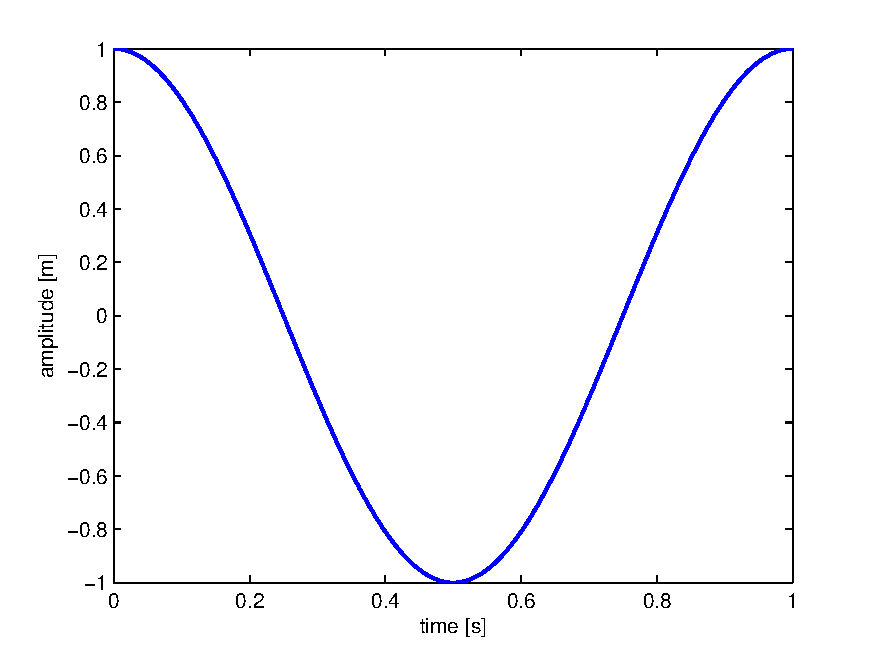
\includegraphics[width=\linewidth]{results}
%\caption{In-text Picture}
%\label{fig:results}
%\end{figure}
%
%Reference to Figure \ref{fig:results}.

%------------------------------------------------


%\begin{table}[hbt]
%\caption{Table of Grades}
%\centering
%\begin{tabular}{llr}
%\toprule
%\multicolumn{2}{c}{Name} \\
%\cmidrule(r){1-2}
%First name & Last Name & Grade \\
%\midrule
%John & Doe & $7.5$ \\
%Richard & Miles & $2$ \\
%\bottomrule
%\end{tabular}
%\label{tab:label}
%\end{table}

%\begin{description}
%\item[Word] Definition
%\item[Concept] Explanation
%\item[Idea] Text
%\end{description}


%\begin{itemize}[noitemsep] % [noitemsep] removes whitespace between the items for a compact look
%\item First item in a list
%\item Second item in a list
%\item Third item in a list
%\end{itemize}


%------------------------------------------------
%\phantomsection
%\section*{Acknowledgments} % The \section*{} command stops section numbering
%
%\addcontentsline{toc}{section}{Acknowledgments} % Adds this section to the table of contents
%
%So long and thanks for all the fish \cite{Figueredo:2009dg}.




\end{document}